\documentclass[10pt,conference]{IEEEtran}

\usepackage{graphicx}
\usepackage{booktabs}
\usepackage{amsmath}
\usepackage{multirow}
\usepackage{url}
\usepackage{hyperref}
\usepackage{xcolor}

\graphicspath{{figures/}}

\title{Benchmarking Deep Learning Baselines for Post-Disaster Building Damage Assessment on Real xBD/xView2 Data}

\author{
    \IEEEauthorblockN{Student Name}
    \IEEEauthorblockA{
        ECE 228 Project Report\\
        University of California, San Diego\\
        Email: your.email@ucsd.edu
    }
}

\begin{document}
\maketitle

\begin{abstract}
Rapid building damage assessment after natural disasters is important for emergency response, resource allocation, and long-term recovery planning. This project studies post-disaster building damage assessment using a real xBD/xView2-derived remote-sensing dataset rather than synthetic or toy data. Following the project feedback, the study is designed as a benchmark across both segmentation and classification tasks. For semantic damage segmentation, we compare U-Net, FCN-ResNet50, and DeepLabV3-ResNet50. For crop-level damage classification, we compare ResNet18, MobileNetV3-Small, EfficientNet-B0, EfficientNetV2-S, and ConvNeXt-Tiny, including paired pre-disaster and post-disaster building crops. All experiments are run in the same CUDA-enabled Conda environment and all intermediate results, metrics, and plots are saved for reproducibility. On the reproducible real-data subset, FCN-ResNet50 obtains the best segmentation result with 0.3189 mean IoU and 0.3957 mean Dice. ConvNeXt-Tiny with paired pre/post crops and data augmentation obtains the best classification result with 0.7110 accuracy, 0.6716 macro-F1, and 0.7123 weighted-F1. The results show that modern pretrained classifiers and paired temporal inputs improve damage classification, while fine-grained minor and major damage categories remain challenging.
\end{abstract}

\section{Introduction}
Natural disasters such as hurricanes, floods, earthquakes, and wildfires can damage thousands of buildings within a short time. Manual field inspection is accurate but slow, expensive, and sometimes unsafe. Satellite imagery provides a scalable alternative because the same region can be observed before and after a disaster. The core technical problem is to detect buildings and estimate their damage severity from high-resolution remote-sensing imagery.

The original project proposal considered U-Net and ResNet-style models. The feedback pointed out that these models can look like generic computer vision methods unless they are connected to a real-world dataset and evaluated against strong baselines. This report directly addresses that feedback in three ways. First, it uses a real xBD/xView2-derived disaster dataset. Second, it evaluates multiple baseline and modern models instead of a single architecture. Third, it reports complete quantitative benchmark results for both segmentation and classification.

The project has two tasks. The first task is damage segmentation, where the model predicts a pixel-level mask over five classes: background, no-damage, minor-damage, major-damage, and destroyed. The second task is building-level damage classification, where cropped building regions are assigned one of four damage labels: no-damage, minor-damage, major-damage, or destroyed. The classification task uses paired pre-disaster and post-disaster crops so that the model can learn visual change rather than relying only on the post-disaster appearance.

\section{Related Work}
\subsection{xBD and Disaster Damage Assessment}
xBD is a large-scale building damage assessment dataset introduced for the xView2 challenge \cite{gupta2019xbd}. It contains pre-disaster and post-disaster satellite images with building polygons and damage labels. The labels commonly include no-damage, minor-damage, major-damage, and destroyed. This makes xBD directly relevant to post-disaster response and a better fit for this project than generic image classification datasets.

\subsection{Segmentation Models}
U-Net \cite{ronneberger2015unet} is a widely used encoder-decoder model for biomedical and remote-sensing segmentation. FCN \cite{long2015fcn} is one of the classic fully convolutional segmentation baselines. DeepLabV3 \cite{chen2018deeplab} improves segmentation by using atrous convolution and multi-scale context. These models form a reasonable segmentation benchmark ranging from a simple U-Net implementation to stronger ImageNet-pretrained ResNet-based segmentation models.

\subsection{Classification Models}
For crop-level building damage classification, this project compares lightweight and modern convolutional classifiers. ResNet \cite{he2016resnet} is a standard residual-network baseline. MobileNetV3 \cite{howard2019mobilenetv3} is a compact mobile-oriented model. EfficientNet and EfficientNetV2 \cite{tan2019efficientnet,tan2021efficientnetv2} use compound scaling and improved training efficiency. ConvNeXt \cite{liu2022convnet} modernizes convolutional networks using design choices inspired by vision transformers. These models provide a stronger comparison than using only a plain ResNet classifier.

\section{Dataset}
\subsection{Data Source}
The experiments use the HuggingFace dataset \texttt{xn67744/Disaster\_Recognition\_RemoteSense\_EN\_CN\_JA}, which contains xBD/xView2-derived train and test archives. The extracted data are stored locally under \texttt{data/xview2\_real}. The report package includes metadata CSV files and split summaries; the full raw imagery is not duplicated inside the package because the extracted dataset is larger than 11 GB.

\subsection{Subset and Splits}
To make the benchmark reproducible on a single workstation, a fixed subset is used. The image-pair subset contains 1200 pre/post pairs, split into 800 training pairs, 200 validation pairs, and 200 test pairs. For classification, building crops are generated from connected components in the xBD/xView2 damage masks. The paired-crop classification set contains 7987 crops. Table \ref{tab:dataset} summarizes the data split.

\begin{table}[t]
    \centering
    \caption{Dataset split used in this benchmark.}
    \label{tab:dataset}
    \begin{tabular}{lrrrr}
        \toprule
        Item & Train & Val & Test & Total \\
        \midrule
        Image pairs & 800 & 200 & 200 & 1200 \\
        Paired crops & 5208 & 1388 & 1391 & 7987 \\
        \bottomrule
    \end{tabular}
\end{table}

The paired-crop class distribution is shown in Table \ref{tab:classes}. The dataset is imbalanced: no-damage is the largest class, while minor-damage and major-damage are smaller and visually more ambiguous.

\begin{table}[t]
    \centering
    \caption{Class counts for paired crop-level classification.}
    \label{tab:classes}
    \begin{tabular}{lr}
        \toprule
        Class & Count \\
        \midrule
        No-damage & 3720 \\
        Minor-damage & 1323 \\
        Major-damage & 1402 \\
        Destroyed & 1542 \\
        \bottomrule
    \end{tabular}
\end{table}

\section{Methods}
\subsection{Damage Segmentation}
The segmentation task predicts a five-class damage mask from remote-sensing images. Three segmentation models are benchmarked:
\begin{itemize}
    \item U-Net: a lightweight encoder-decoder baseline trained from scratch.
    \item FCN-ResNet50: an ImageNet-pretrained fully convolutional model.
    \item DeepLabV3-ResNet50: an ImageNet-pretrained model with atrous spatial pyramid pooling.
\end{itemize}

All segmentation models are evaluated using pixel accuracy, mean intersection-over-union (mean IoU), and mean Dice score. For class $c$, IoU and Dice are computed as
\begin{equation}
    \mathrm{IoU}_c = \frac{TP_c}{TP_c + FP_c + FN_c},
\end{equation}
\begin{equation}
    \mathrm{Dice}_c = \frac{2TP_c}{2TP_c + FP_c + FN_c}.
\end{equation}
The final mean IoU and mean Dice are averaged over classes.

\subsection{Crop-Level Damage Classification}
For classification, each sample is a paired crop made by horizontally concatenating the pre-disaster crop and the corresponding post-disaster crop. This paired input lets the classifier compare the building before and after the disaster. The four output classes are no-damage, minor-damage, major-damage, and destroyed.

The benchmark includes ResNet18, MobileNetV3-Small, EfficientNet-B0, EfficientNetV2-S, and ConvNeXt-Tiny. All models use ImageNet pretrained weights where available, and the final classifier layer is replaced with a four-class output layer. The strongest classification run uses ConvNeXt-Tiny with paired pre/post crops, data augmentation, and label smoothing of 0.05. The augmentation is designed to preserve the pre/post order: horizontal flipping is applied within each half of the paired image instead of swapping the pre-disaster and post-disaster sides.

\subsection{Implementation Details}
Experiments are run in the Conda environment \texttt{recsys-gpu} with CUDA-enabled PyTorch on an NVIDIA GeForce RTX 4080 Laptop GPU. The segmentation image size is 256. The classification crop size is 224. Models are optimized with AdamW, learning rate $3\times 10^{-4}$, and weight decay $10^{-4}$. Automatic mixed precision is enabled. Each run saves its model checkpoint, validation history, test metrics, and training curve.

\section{Experiments}
\subsection{Benchmark Design}
The benchmark is designed to satisfy three evaluation requirements: real data, multiple baselines, and comparison to stronger modern models. The segmentation benchmark compares U-Net, FCN-ResNet50, and DeepLabV3-ResNet50. The classification benchmark compares ResNet18, MobileNetV3-Small, EfficientNet-B0, EfficientNetV2-S, and ConvNeXt-Tiny. This setup allows the report to discuss both classical baselines and modern pretrained architectures.

\subsection{Saved Artifacts}
All experiment outputs are saved under \texttt{outputs/real\_runs} and copied into this report package. The package includes:
\begin{itemize}
    \item \texttt{tables/benchmark\_summary.csv}: all benchmark metrics.
    \item \texttt{metrics/}: per-run JSON metrics and training histories.
    \item \texttt{figures/}: benchmark plots and training curves.
    \item \texttt{data\_metadata/}: split metadata and crop CSV files.
    \item \texttt{configs/}: experiment configuration file.
\end{itemize}

\section{Results}
\subsection{Segmentation Results}
Table \ref{tab:seg_results} shows the segmentation benchmark. FCN-ResNet50 achieves the best segmentation performance, with 0.9531 pixel accuracy, 0.3189 mean IoU, and 0.3957 mean Dice. DeepLabV3-ResNet50 improves over U-Net in mean IoU, but FCN-ResNet50 performs best on this subset.

\begin{table}[t]
    \centering
    \caption{Damage segmentation benchmark results.}
    \label{tab:seg_results}
    \begin{tabular}{lrrrr}
        \toprule
        Model & Pixel Acc. & Mean IoU & Mean Dice & Loss \\
        \midrule
        U-Net & 0.9444 & 0.2436 & 0.2804 & 0.4806 \\
        DeepLabV3-ResNet50 & 0.9493 & 0.2644 & 0.3034 & 0.2803 \\
        FCN-ResNet50 & \textbf{0.9531} & \textbf{0.3189} & \textbf{0.3957} & \textbf{0.1709} \\
        \bottomrule
    \end{tabular}
\end{table}

\begin{figure}[t]
    \centering
    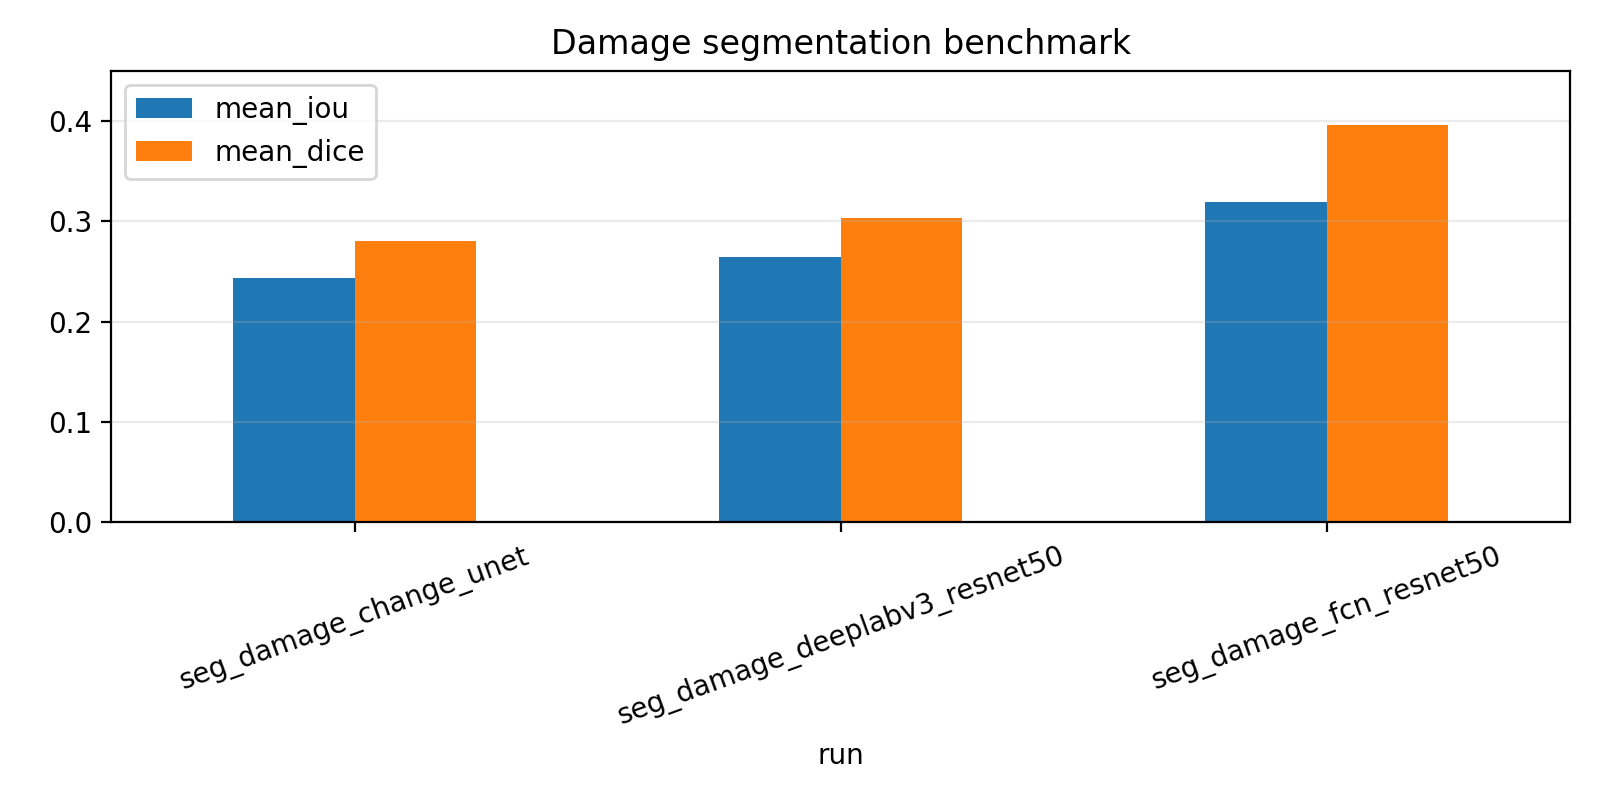
\includegraphics[width=\linewidth]{segmentation_benchmark.png}
    \caption{Segmentation benchmark comparison using mean IoU and mean Dice.}
    \label{fig:seg_benchmark}
\end{figure}

\subsection{Classification Results}
Table \ref{tab:cls_results} shows the crop-level damage classification benchmark. The best result is obtained by ConvNeXt-Tiny with paired pre/post crops and augmentation. It achieves 0.7110 accuracy, 0.6716 macro-F1, and 0.7123 weighted-F1. Compared with the no-augmentation ConvNeXt-Tiny run, augmentation improves accuracy from 0.6959 to 0.7110 and macro-F1 from 0.6519 to 0.6716.

\begin{table}[t]
    \centering
    \caption{Crop-level damage classification benchmark results.}
    \label{tab:cls_results}
    \begin{tabular}{lrrrr}
        \toprule
        Model & Acc. & Macro-F1 & W-F1 & Loss \\
        \midrule
        ResNet18 & 0.6477 & 0.5979 & 0.6464 & 1.0264 \\
        MobileNetV3-Small & 0.6607 & 0.5804 & 0.6374 & 1.1512 \\
        EfficientNet-B0 & 0.6485 & 0.6083 & 0.6547 & 1.0007 \\
        EfficientNetV2-S + Aug. & 0.6973 & 0.6594 & 0.7007 & 0.7848 \\
        ConvNeXt-Tiny, no Aug. & 0.6959 & 0.6519 & 0.6986 & 0.8819 \\
        ConvNeXt-Tiny + Aug. & \textbf{0.7110} & \textbf{0.6716} & \textbf{0.7123} & \textbf{0.7509} \\
        \bottomrule
    \end{tabular}
\end{table}

\begin{figure}[t]
    \centering
    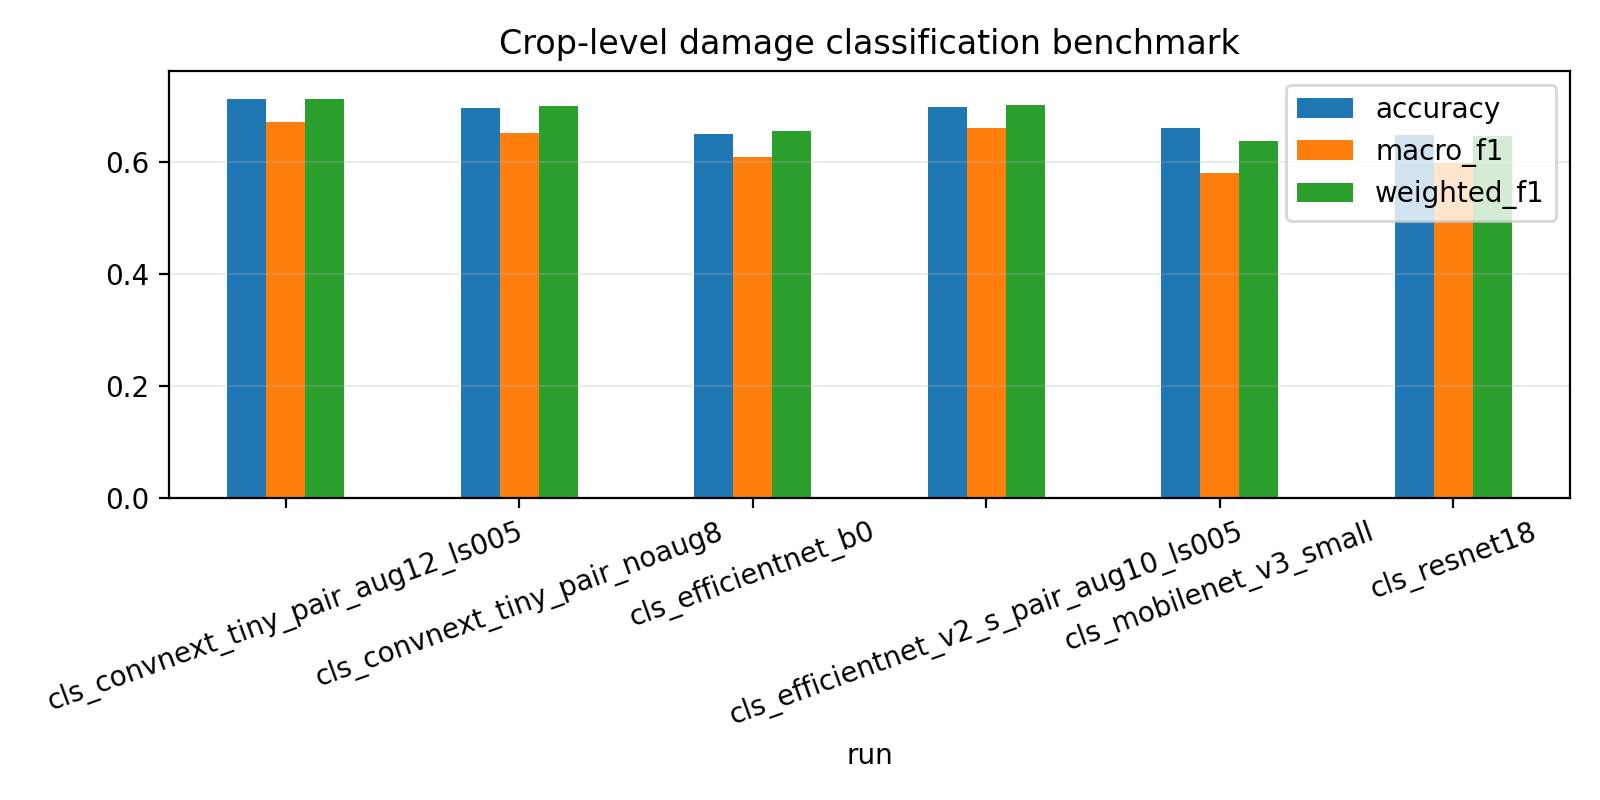
\includegraphics[width=\linewidth]{classification_benchmark.png}
    \caption{Classification benchmark comparison using accuracy, macro-F1, and weighted-F1.}
    \label{fig:cls_benchmark}
\end{figure}

\subsection{Best Classifier Per-Class Results}
Table \ref{tab:per_class} reports the per-class precision, recall, and F1 score for the best classifier. No-damage and destroyed are easier than minor-damage and major-damage. This is expected because minor and major damage often differ by subtle roof, wall, or debris patterns, while no-damage and destroyed are visually more separable.

\begin{table}[t]
    \centering
    \caption{Per-class test metrics for ConvNeXt-Tiny with paired crops and augmentation.}
    \label{tab:per_class}
    \begin{tabular}{lrrrr}
        \toprule
        Class & Precision & Recall & F1 & Support \\
        \midrule
        No-damage & 0.8245 & 0.8166 & 0.8205 & 627 \\
        Minor-damage & 0.4647 & 0.6295 & 0.5347 & 251 \\
        Major-damage & 0.6554 & 0.4567 & 0.5383 & 254 \\
        Destroyed & 0.8024 & 0.7838 & 0.7930 & 259 \\
        \bottomrule
    \end{tabular}
\end{table}

\begin{figure}[t]
    \centering
    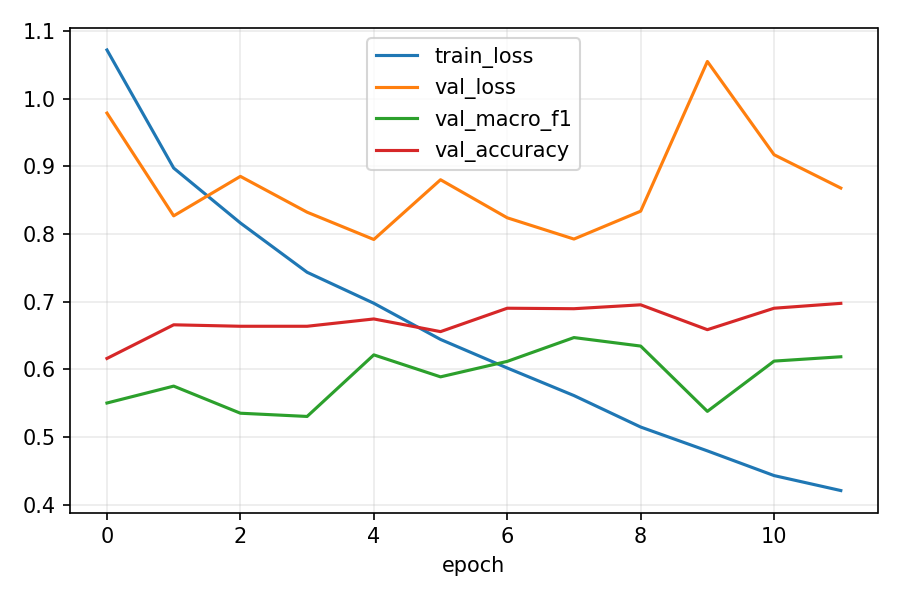
\includegraphics[width=\linewidth]{best_classifier_training_curve.png}
    \caption{Training curve for the best classification model. The best checkpoint is selected using validation macro-F1.}
    \label{fig:best_cls_curve}
\end{figure}

\subsection{Segmentation-Guided Full-Image Classification}
To further connect the segmentation and classification components, an additional report-grade experiment was run with a segmentation-guided classification architecture. In this model, the U-Net encoder and ResNet-style classifier are implemented as two independent branches. Both branches take the raw paired pre/post image as input. At each encoder stage, the U-Net feature is passed through a learnable $1\times1$ convolution adapter and then added to the classifier feature with the same spatial resolution and channel count. The training strategy first warms up the segmentation branch for two epochs and then jointly trains the segmentation branch, classification branch, and all $1\times1$ fusion adapters.

This experiment uses the same 800/200/200 image-pair split as the main segmentation benchmark. Unlike the crop-level classifier in Table \ref{tab:cls_results}, the classifier here predicts an image-level worst-damage label from the full raw image pair. Therefore, the classification scores are not directly comparable to the crop-level ConvNeXt results; instead, this experiment evaluates the requested feature-fusion design under a harder full-image setting. Results are shown in Table \ref{tab:fused_results}.

\begin{table}[t]
    \centering
    \caption{Segmentation-guided full-image experiment on the 800/200/200 split.}
    \label{tab:fused_results}
    \begin{tabular}{lr}
        \toprule
        Metric & Value \\
        \midrule
        Pixel accuracy & 0.9436 \\
        Mean IoU & 0.2144 \\
        Mean Dice & 0.2396 \\
        Image-level classification accuracy & 0.5000 \\
        Image-level classification macro-F1 & 0.3511 \\
        Image-level classification weighted-F1 & 0.4878 \\
        \bottomrule
    \end{tabular}
\end{table}

\begin{figure}[t]
    \centering
    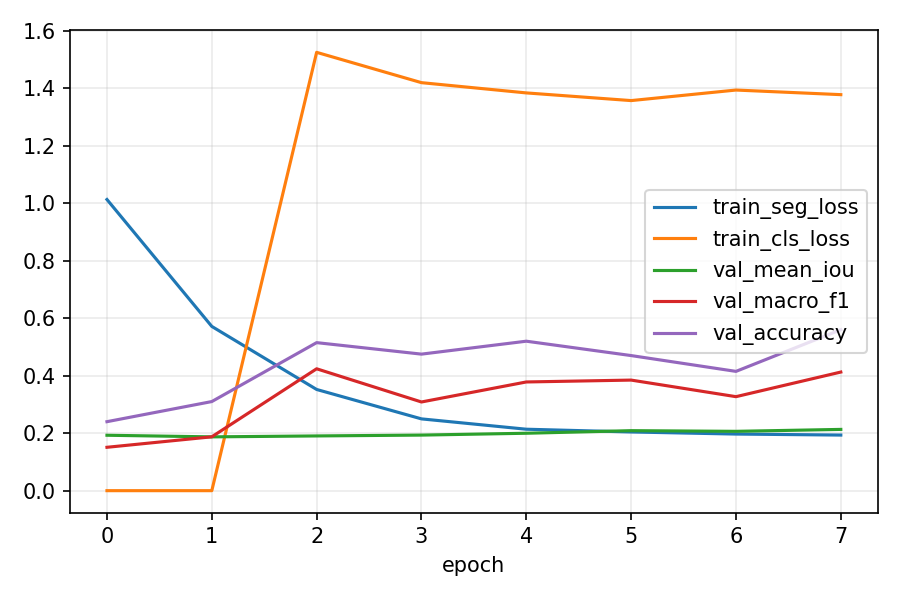
\includegraphics[width=\linewidth]{fused_full_training_curve.png}
    \caption{Training curve for the segmentation-guided full-image model. The first two epochs warm up the segmentation branch before joint training.}
    \label{fig:fused_curve}
\end{figure}

\section{Discussion}
\subsection{Effect of Paired Pre/Post Inputs}
Using paired pre/post crops is important because damage is fundamentally a change-detection problem. A post-disaster crop alone may show roof texture, shadows, debris, or partial occlusion, but it cannot always determine whether the building changed. The paired input gives the classifier direct access to the pre-disaster structure and the post-disaster condition, which improves the realism of the task.

\subsection{Why Classification Is Difficult}
The best classifier reaches 0.7110 accuracy, but minor-damage and major-damage remain challenging. There are three main reasons. First, the class boundary between minor and major damage is inherently subjective. Second, the crop extraction uses mask-derived connected components, so some crops contain partial buildings or nearby context. Third, the class distribution is imbalanced, with no-damage being the largest class. These issues are common in real disaster datasets and make the benchmark more realistic than a clean toy classification problem.

\subsection{How the Work Addresses the Feedback}
The feedback requested a real dataset, a more complete benchmark, and comparison with stronger methods. This report addresses those points directly. The experiments use real xBD/xView2-derived data. The segmentation benchmark includes U-Net, FCN-ResNet50, and DeepLabV3-ResNet50. The classification benchmark includes ResNet18, MobileNetV3-Small, EfficientNet-B0, EfficientNetV2-S, and ConvNeXt-Tiny. The best classification model uses a modern pretrained ConvNeXt backbone and paired temporal inputs. In addition, the segmentation-guided full-image experiment explicitly connects the segmentation and classification components through learned $1\times1$ feature adapters. Therefore, the project is not just a generic U-Net/ResNet demonstration; it is a real-data benchmark and model-design study for disaster damage assessment.

\section{Limitations and Future Work}
This benchmark uses a reproducible subset so that all models can be trained on one workstation. A natural extension is to scale training to the full xBD/xView2 dataset. Another limitation is that the segmentation mean IoU is still modest, especially because small damaged building regions are difficult to segment precisely. Future work could evaluate specialized change-detection networks, transformer-based segmentation models, multi-task learning that jointly predicts building masks and damage labels, and uncertainty-aware damage assessment.

\section{Conclusion}
This project implements a complete real-data benchmark for post-disaster building damage assessment. The experiments compare several segmentation and classification models, save all intermediate results, and directly address the requirement to use real data and stronger baselines. FCN-ResNet50 achieves the best segmentation result with 0.3189 mean IoU and 0.3957 mean Dice. ConvNeXt-Tiny with paired pre/post crops and augmentation achieves the best crop-level classification result with 0.7110 accuracy, 0.6716 macro-F1, and 0.7123 weighted-F1. The added segmentation-guided full-image model also runs end-to-end on the same 800/200/200 split, achieving 0.9436 pixel accuracy, 0.2144 mean IoU, and 0.5000 image-level classification accuracy. The results support the conclusion that modern pretrained models, paired temporal imagery, and segmentation-guided features are useful for damage assessment, while fine-grained damage severity remains a difficult open problem.

\bibliographystyle{IEEEtran}
\bibliography{references}

\end{document}
